\documentclass[handout]{beamer}
\usepackage[utf8]{inputenc}
\usetheme{metropolis}           % Use metropolis theme
\title{Algorithmique Avancée}
\subtitle{Structures de données : Première Partie}
\date{Année académique 2017 -- 2018}
\author{Julien Roland}

\let\emph\relax % there's no \RedeclareTextFontCommand
\DeclareTextFontCommand{\emph}{\bfseries\em}

\usepackage{amsmath}
\newcommand{\Op}[2]{\texttt{\underline{#1}#2}}

\newcommand{\N}{\mathbb{N}}
\newcommand{\R}{\mathbb{R}}

\usepackage{listings}
\usepackage{algorithmicx}
\usepackage{algpseudocode}
\usepackage{hyperref}

\begin{document}
\lstset{language=c++, basicstyle=\small, columns=fullflexible}
    
\setbeamercovered{dynamic}
    
\maketitle

\begin{frame}[fragile]{ADT Dictionaire} 
	Un dictionaire est un \emph{ensemble dynamique} contenant les éléments représentés par un objet composé d'un ou plusieurs attributs. Par exemple :
	\begin{lstlisting}
    template<typename Key, typename T>
    struct Element {
        Key key;
        T value;
    };
	\end{lstlisting}
	Opérations définies sur un dictionnaire D:
	\begin{itemize}
		\item \lstinline{Search(D, k)} : retourne un pointeur vers un élément dont la valeur de \textit{key} est égale à $k$, sinon NULL.
		\item \lstinline{Insert(D, x)} : ajout de l'élément pointé par $x$
		\item \lstinline{Delete(D, x)} : supprime l'élément pointé par $x$
	\end{itemize}
\end{frame}

\begin{frame}[fragile]{Exercices}
	\begin{enumerate}
		\item Comparer la complexité au pire cas des opérations de l'ADT dictionnaire implémenté avec les conteneurs suivants : liste simplement chaînée, liste simplement chaînée triée, liste doublement chaînée, liste doublement chaînée triée.
	\end{enumerate}
\end{frame}

\begin{frame}[t]{Gestion Mémoire}
	Vision simplifiée de l'espace d'adressage d'un processus :
	\begin{center}
		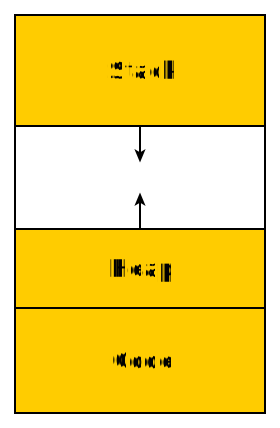
\includegraphics[scale=0.4]{figures/memory_layout.pdf}
	\end{center}
\end{frame}

\begin{frame}[t]{Stack}
	\vfill
	\begin{columns}
		\begin{column}{0.45\textwidth}
			Chaque appel de fonction mène à la création d'un cadre de pile (\emph{stack frame}) contenant:
			\begin{itemize}
				\item \emph{Variables automatiques}: arguments et variables locales automatiquement crées lors d'un appel de fonction.
				\item \emph{Adresse de retour}: ajoutée au cadre courant avant un nouvel appel.
			\end{itemize}
		\end{column}
		\begin{column}{0.45\textwidth}
			Le Stack contient le contexte d'exécution:
			\begin{center}
				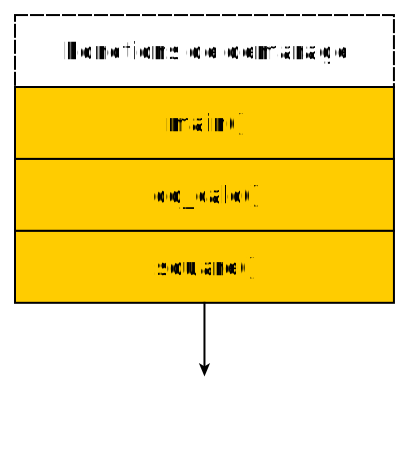
\includegraphics[scale=0.4]{figures/execution_stack.pdf}
			\end{center}
		\end{column}
	\end{columns}    
	\vfill
\end{frame}

\begin{frame}[fragile]{Stack}
	\vfill
	\begin{columns}
		\begin{column}{0.45\textwidth}
			\begin{lstlisting}
int square(int x) {
    int result = x * x;
    return result;
}

void do_calc(int val) {
    std::cout << "The square of "
              << val
              << " is ",
              << square(val) << '\n';
}

int main() {
    static int key = 9973
    do_calc(key);
    return 0;
}
			\end{lstlisting}
		\end{column}
		\begin{column}{0.45\textwidth}
			Le Stack contient le contexte d'exécution:
			\begin{center}
				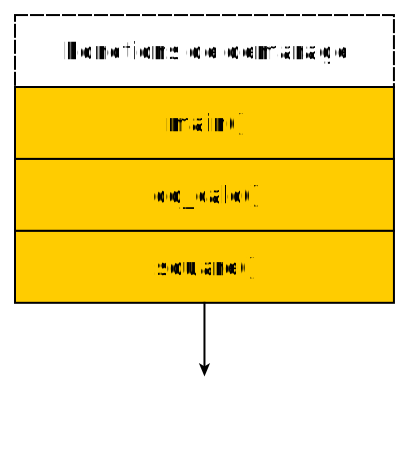
\includegraphics[scale=0.4]{figures/execution_stack.pdf}
			\end{center}
		\end{column}
	\end{columns}    
	\vfill
\end{frame}

\begin{frame}[t]{Stack et Heap : en détails}
	\begin{itemize}
		\item \emph{Stack (Pile):} Composé de \emph{stack frames} ajoutés au sommet du stack à chaque appel de fonction. Elles contiennent les \emph{variables locales} (automatiques)  et \emph{paramètres} de la \emph{fonction}. Le pointeur d'instruction (adresse de retour dans le code) ainsi que les registres y sont également sauvegardés avant un appel de fonction. Ceux-ci sont utilisés afin de restaurer le contexte d'exécution après un retour de fonction.
		\item \emph{Heap (Tas):} Espace mémoire utilisé lors de l'allocation de blocs mémoire par une expression telle que \lstinline{new int[100]}. Des objets créés par une telle expression ont une durée de vie qui ne dépend pas de la portée. 
	\end{itemize}
\end{frame}

\begin{frame}[fragile]{Données contiguës et liées}
	\vfill
	\begin{columns}
		\begin{column}{0.35\textwidth}
			\begin{lstlisting}
class Data;

void f() {
    std::vector<Data> v(30);
    // ...
}
			\end{lstlisting}
		\end{column}
		\begin{column}{0.55\textwidth}
			\begin{center}
				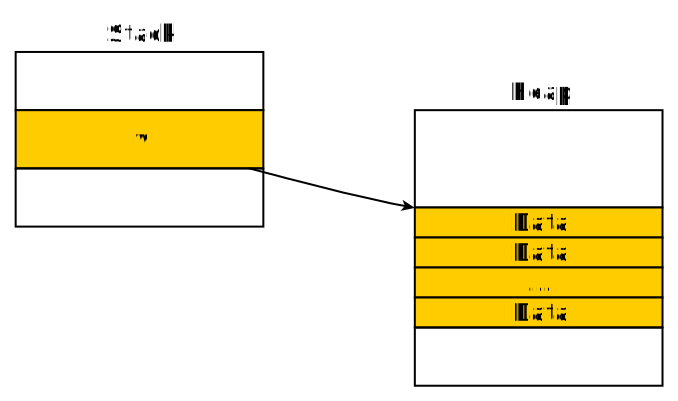
\includegraphics[scale=0.25]{figures/contiguous_data.pdf}
			\end{center}
		\end{column}
	\end{columns}    
	\vfill
\end{frame}

\begin{frame}[fragile]{Données contiguës et liées}
	\vfill
	\begin{columns}
		\begin{column}{0.5\textwidth}
			\begin{lstlisting}
class Data;

void f() {
    std::vector<data*> v;
    v.push_pack(new Data());
    // ...
}
			\end{lstlisting}
		\end{column}
		\begin{column}{0.55\textwidth}
			\begin{center}
				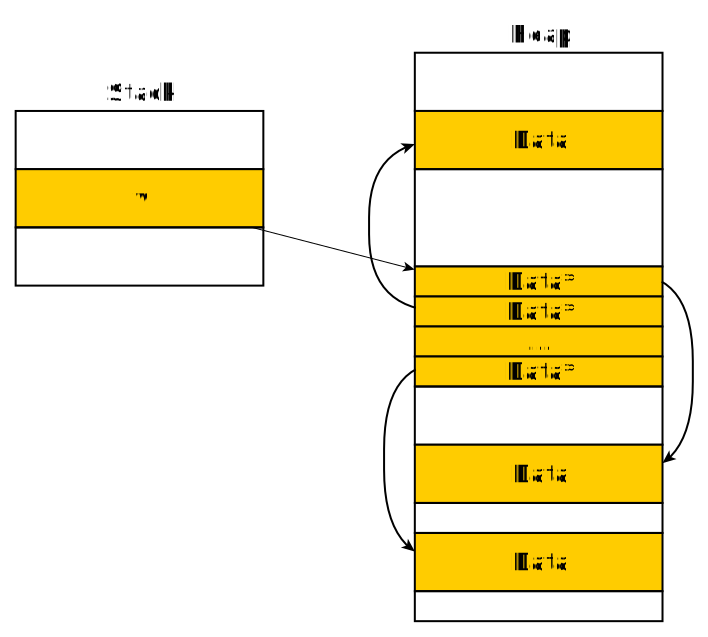
\includegraphics[scale=0.25]{figures/contiguous_data_pointers.pdf}
			\end{center}
		\end{column}
	\end{columns}    
	\vfill
\end{frame}

\begin{frame}[fragile]{Données contiguës et liées}
	\vfill
	\begin{columns}
		\begin{column}{0.35\textwidth}
			\begin{lstlisting}
class Data;

void f() {
    std::list<Data> list;
    list.emplace_back();
    // ...
}
			\end{lstlisting}
		\end{column}
		\begin{column}{0.55\textwidth}
			\begin{center}
				Vision idéalisée :
				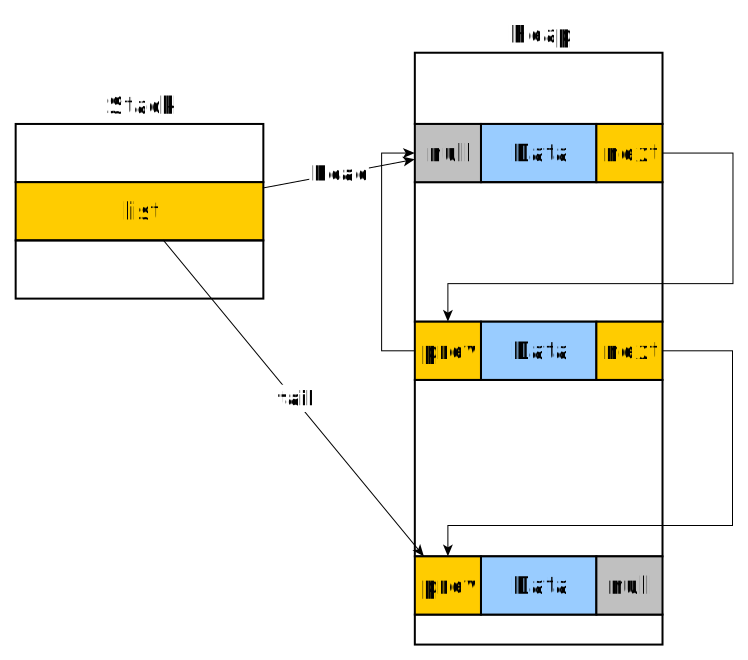
\includegraphics[scale=0.25]{figures/linked_data.pdf}
			\end{center}
		\end{column}
	\end{columns}    
	\vfill
\end{frame}

\begin{frame}[fragile]{Données contiguës et liées}
	\vfill
	\begin{columns}
		\begin{column}{0.35\textwidth}
			\begin{lstlisting}
class Data;

void f() {
    std::list<Data*> list;
    list.push_back(new Data());
    // ...
}
			\end{lstlisting}
		\end{column}
		\begin{column}{0.55\textwidth}
			\begin{center}
				Vision idéalisée :
				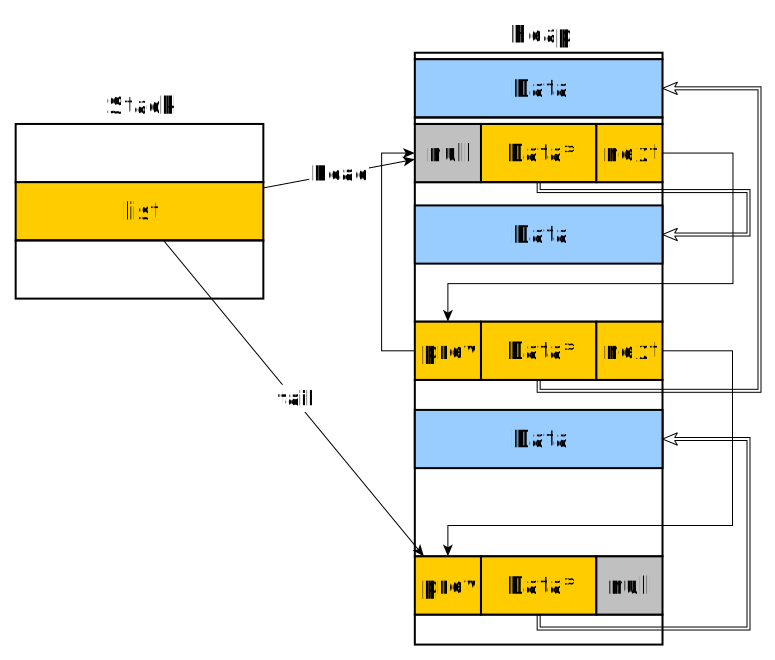
\includegraphics[scale=0.25]{figures/linked_data_pointer.pdf}
			\end{center}
		\end{column}
	\end{columns}    
	\vfill
\end{frame}

\begin{frame}[fragile]{Structures de données contiguës}
	Les structures de données contiguës telles que les tableaux sont composés d'une seule portion de mémoire dans l'espace d'adressage du processus.\\
	\vfill
	\emph{Avantages:}
	\begin{itemize}
		\item Accès direct à un élément.
		\item Utilisation efficace de la mémoire (par exemple, pas de pointeurs \textit{prev} et \textit{next}.)
		\item Localité mémoire, pouvoir tirer partie de la proximité en mémoire lors d'un parcours séquentiel des données (utilisation du cache CPU)
	\end{itemize}
	\emph{Désavantage:}
	\begin{itemize}
		\item Coût important pour augmenter ou diminuer la taille de la structure.
	\end{itemize}
\end{frame}

\begin{frame}[fragile]{ADT : File à priorité (priority queue)}
	Une file à priorité est un conteneur d'éléments, chacun associé à une \emph{clé}. Les opérations fondamentales pour une file à priorité \lstinline{P} :
	\begin{itemize}
		\item \lstinline{insert(P, e)} : insertion de l'élément e dans P.
		\item \lstinline{min(P)} : retourne un élément de P avec la plus petite valeur de clé (relation d'ordre : $\leqslant$). 
		\item \lstinline{remove_min(P)} : supprime de P l'élément \lstinline{min(P)}
	\end{itemize}

	Quelles implémentations ?
\end{frame}

\begin{frame}[fragile]{Tas binaire : Arbre binaire complet}
	Une manière efficace d'implémenter une file à priorité consiste à utiliser un \emph{tas binaire}.
	\vfill
	\begin{columns}
		\begin{column}{0.55\textwidth}
			Un tas binaire est un \emph{arbre binaire complet}:
			\begin{itemize}
				\item Chaque niveau, excepté (éventuellement) le dernier est complètement rempli.
				\item Le dernier niveau est rempli de gauche à droite.
			\end{itemize}
		\end{column}
		\begin{column}{0.45\textwidth}
			\centering
			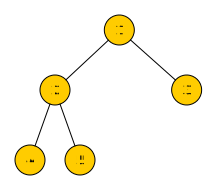
\includegraphics[scale=0.7]{figures/arbre_binaire_complet.pdf}
		\end{column}
	\end{columns}
\end{frame}

\begin{frame}[fragile]{Tas binaire : propriété relationnelle}
	Un tas binaire satisfait la propriété relationnelle suivante: \textit{pour tout noeud v autre que la racine, la clé associée à v est plus grande ou égale à la clé associée au parent de v}.
	\vfill
	\begin{columns}
		\begin{column}{0.45\textwidth}
			\Large
			$$
			\left\{\begin{array}{l}
			x \leqslant y\\
			x \leqslant z
			\end{array}\right.
			$$
		\end{column}
		\begin{column}{0.45\textwidth}
			\centering
			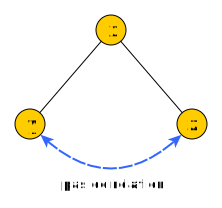
\includegraphics[scale=0.7]{figures/tas_binaire_relation.pdf}
		\end{column}
	\end{columns}
\end{frame}

\begin{frame}[fragile]{Tas binaire}
	\begin{center}
		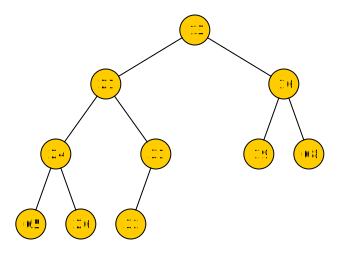
\includegraphics[scale=0.6]{figures/tas_binaire.pdf}
	\end{center}
	\vfill
\end{frame}

\begin{frame}[fragile]{Tas binaire : insertion}
	\begin{center}
		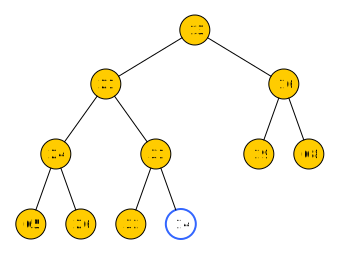
\includegraphics[scale=0.6]{figures/tas_binaire_insertion_t1.pdf}
	\end{center}
	Insertion en fin de l'arbre afin de maintenir un arbre complet.
\end{frame}

\begin{frame}[fragile]{Tas binaire : insertion}
	\begin{center}
		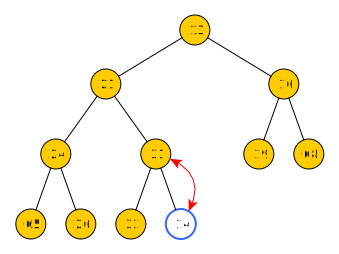
\includegraphics[scale=0.6]{figures/tas_binaire_insertion_t2.pdf}
	\end{center}
	Si le nouveau noeud est un fils droit et que sa valeur est $<$ à celle du parent alors cela implique que cette valeur est $<$ à celle du fils gauche. Pourquoi ?
\end{frame}

\begin{frame}[t]{Tas binaire : insertion}
	\begin{figure}
		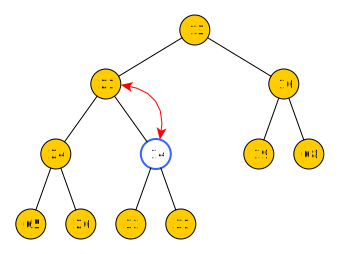
\includegraphics[scale=0.6]{figures/tas_binaire_insertion_t3.pdf}
	\end{figure}
\end{frame}

\begin{frame}[t]{Tas binaire : insertion}
	\begin{figure}
		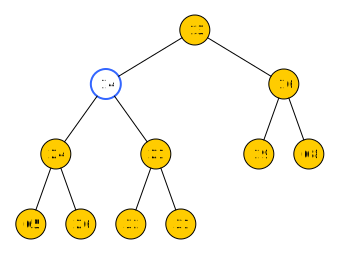
\includegraphics[scale=0.6]{figures/tas_binaire_insertion_t4.pdf}
	\end{figure}
	Fin de l'algorithme : l'arbre binaire est complet et satisfait à nouveau la propriété relationnelle.
	\vfill
\end{frame}

\begin{frame}[fragile]{Tas binaire : insertion}
	\emph{Pseudo-code:}
	\begin{enumerate}
		\item Ajouter le nouvel élément à la fin de l'arbre complet $\Rightarrow$ le noeud $z$.
		\item Si le noeud $z$ est à la racine de l'arbre $\Rightarrow$ \emph{fin}, sinon aller en 3.
		\item Soit $u$, le noeud parent de $z$, si $key(z) \geqslant key(u)$, alors $\emph{fin}$, sinon échanger les noeuds $z$ et $z$, aller en 2.
	\end{enumerate}
	L'opération de \emph{percolate-up} (percolation vers le haut) est composé des étapes 2-3.
\end{frame}

\begin{frame}[fragile]{Tas binaire : suppression du minimum}
	\begin{center}
		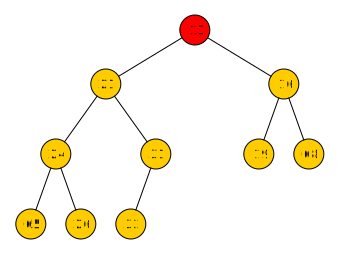
\includegraphics[scale=0.7]{figures/tas_binaire_suppression_min_t1.pdf}
	\end{center}
\end{frame}

\begin{frame}[fragile]{Tas binaire : suppression du minimum}
	\begin{center}
		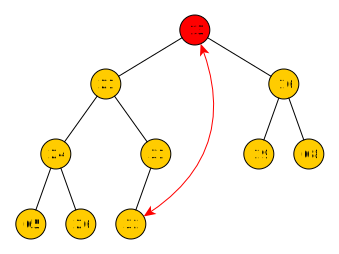
\includegraphics[scale=0.7]{figures/tas_binaire_suppression_min_t2.pdf}
	\end{center}
\end{frame}

\begin{frame}[fragile]{Tas binaire : suppression du minimum}
	\begin{center}
		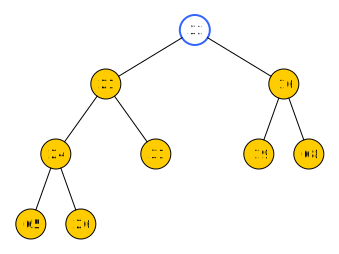
\includegraphics[scale=0.7]{figures/tas_binaire_suppression_min_t3.pdf}
	\end{center}
\end{frame}

\begin{frame}[fragile]{Tas binaire : suppression du minimum}
	\begin{center}
		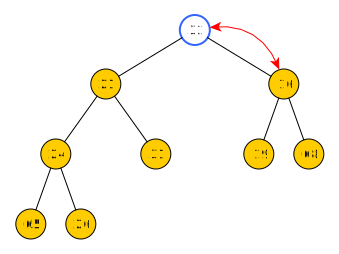
\includegraphics[scale=0.7]{figures/tas_binaire_suppression_min_t4.pdf}
	\end{center}
\end{frame}

\begin{frame}[fragile]{Tas binaire : suppression du minimum}
	\begin{center}
		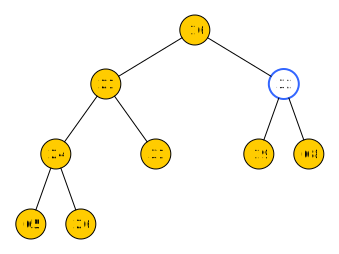
\includegraphics[scale=0.7]{figures/tas_binaire_suppression_min_t5.pdf}
	\end{center}
\end{frame}

\begin{frame}[fragile]{Tas binaire : suppression du minimum}
	\begin{center}
		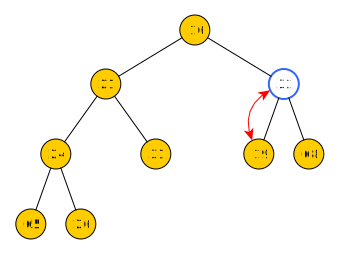
\includegraphics[scale=0.7]{figures/tas_binaire_suppression_min_t6.pdf}
	\end{center}
\end{frame}

\begin{frame}[fragile]{Tas binaire : suppression du minimum}
	\begin{center}
		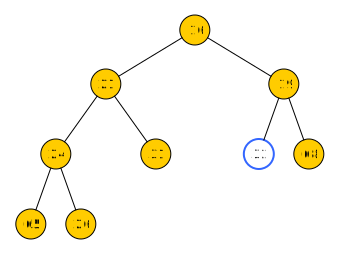
\includegraphics[scale=0.7]{figures/tas_binaire_suppression_min_t7.pdf}
	\end{center}
\end{frame}

\begin{frame}[fragile]{Tas binaire : suppression du minimum}
	\emph{Pseudo-code:}
	\begin{enumerate}
		\item \emph{Si} la taille du heap $> 1$, \emph{alors} remplacer la racine par le dernier noeud de l'arbre afin de conserver un arbre complet, \emph{sinon} supprimer la racine $\Rightarrow$ \emph{fin}.
		\item Soit $z$ la racine de l'arbre. \emph{Si} $z$ est le seul noeud de l'arbre, \emph{alors fin}, \emph{sinon}, aller en 3.
		\item \emph{Si} $z$ n'a pas de fils droit, \emph{alors} notons $s$ le fils gauche de $z$, \emph{sinon} notons $s$, le fils de $z$ avec la plus petite valeur de clé.
		\item \emph{Si} $key(z) \leqslant key(s)$, \emph{alors fin}. \emph{Sinon}, on échange les noeuds $z$ et $s$.
		\item \emph{Si} le sous-arbre de racine $z$ est de taille $> 1$, \emph{alors} aller en 3. \emph{Sinon fin}.
	\end{enumerate}
	L'opération de \emph{percolate-down} (percolation vers le bas) est composée des étapes 3-5.
\end{frame}

\begin{frame}[fragile]{Rappels : partie entière}
	\begin{itemize}
		\item Partie entière par défaut (fonction plancher):
		      $$\lfloor x \rfloor \leqslant x < \lfloor x \rfloor + 1$$
		\item Partie entière par excès (fonction plafond):
		      $$\lceil x \rceil - 1 < x \leqslant \lceil x \rceil$$
	\end{itemize}

	Ne pas confondre avec la \textit{troncature} qui est différente de la partie entière pour les nombres négatifs.
	\vfill
	L'article \textit{wikipedia} suivant résume ces différents concepts: \href{https://fr.wikipedia.org/wiki/Partie_enti%C3%A8re_et_partie_fractionnaire}{fr.wikipedia.org/wiki/Partie\_entière\_et\_partie\_fractionnaire}
\end{frame}

\begin{frame}[fragile]{Tas binaire : analyse de complexité}
	\begin{itemize}
		\item La \emph{hauteur d'un noeud} v est la longueur du chemin joignant la racine à ce noeud. 
		\item La \emph{hauteur d'un arbre} est égale à la hauteur maximale d'un noeud appartenant à cet arbre.
		\item L'ensemble des noeuds à hauteur $i$ est le i-ème \emph{niveau} de l'arbre.
	\end{itemize}
\end{frame}

\begin{frame}[fragile]{Tas binaire : analyse de complexité}
	Étant donné $n$, le nombre de noeuds d'un tas binaire. Quelle est la hauteur $h$ de cet arbre ?
	\begin{center}
		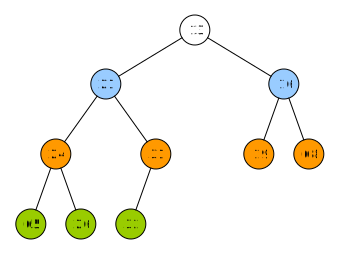
\includegraphics[scale=0.5]{figures/arbre_binaire_complet_niv.pdf}
	\end{center}
	\begin{itemize}
		\item au niveau $i$ (avec $0 \leqslant i \leqslant h-1$) : $2^i$ noeuds
		\item au niveau $h$ : au moins 1 noeud
	\end{itemize}
\end{frame}

\begin{frame}[fragile]{Tas binaire : analyse de complexité}
	Étant donné $n$, le nombre de noeuds d'un tas binaire. Quelle est la hauteur $h$ de cet arbre ?
	\begin{itemize}
		\item Déterminer des bornes supérieures et inférieures sur le nombre de noeuds dans un arbre de hauteur $h$.
		\item Comment déduire de ces bornes que $h = \lfloor \log_2(n) \rfloor$
		\item Sur base de ce résultat déterminer les complexités des opérations de l'ADT file à priorité implémenté avec un tas binaire.
	\end{itemize}
\end{frame}

\begin{frame}[fragile]{Implémentation à l'aide d'un tableau}
	\begin{center}
		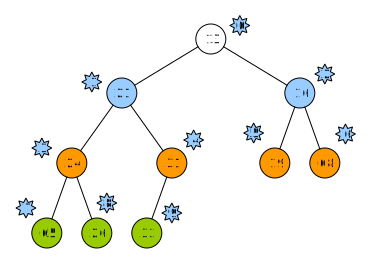
\includegraphics[scale=0.6]{figures/arbre_binaire_complet_index.pdf}\\
		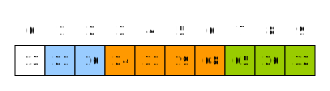
\includegraphics[scale=0.6]{figures/arbre_binaire_complet_tab.pdf}
	\end{center}
\end{frame}

\begin{frame}[fragile]{Implémentation à l'aide d'un tableau}
	\begin{columns}
		\begin{column}{0.45\textwidth}
			\centering
			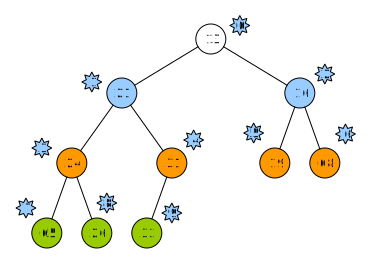
\includegraphics[scale=0.5]{figures/arbre_binaire_complet_index.pdf}\\
			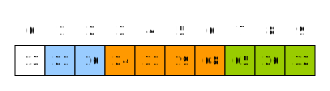
\includegraphics[scale=0.5]{figures/arbre_binaire_complet_tab.pdf}
		\end{column}
		\begin{column}{0.45\textwidth}
			\centering
			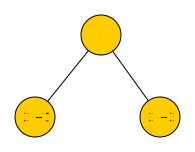
\includegraphics[scale=0.5]{figures/arbre_parent_enfants_index.pdf}
			\begin{itemize}
				\item Comment justifier ce calcul d'indices ?
				\item Comment déterminer la position du parent pour un noeud $i$ ?
			\end{itemize}
		\end{column}
	\end{columns}
\end{frame}

\begin{frame}[t]{Exercices}
\begin{itemize}
	\item Dessiner le tas binaire qui résulte de l'insertion de 10, 12, 1, 14, 6, 5, 8, 15, 3, 9, 7 dans cet ordre, dans un tas binaire initialement vide. Expliciter chaque étape.
	\item Dessiner le tas binaire obtenu après trois \lstinline{remove_min} sur le tas binaire obtenu dans l'exercice précédent. Expliciter chaque étape.
	\item Quelle est la complexité au pire case des trois opérations élémentaires de la file à priorité (\lstinline{insert}, \lstinline{min} et \lstinline{remove_min}) lorsque celle-ci est implémentée à l'aide d'un tableau trié ou un tableau non trié (dont l'espace mémoire réservé est géré de manière dynamique)?
\end{itemize}
\end{frame}

\end{document}